\section{1. Introduction}\label{introduction}

Since 1994, when the FOMC first began announcing its policy decision on the day of the meeting, and especially since 2005, when the statement became a structured instrument of guidance rather than a summary of action, the Federal Reserve's press release has been the primary vehicle through which monetary policy is communicated. By the zero-lower-bound era the statement had become, in a precise sense, the policy itself: with the instruments exhausted, what remained to move was the committee's language. Yet the economics of that language --- what it moves, when, and through which channel --- remains contested. This paper answers the question with an identification rather than a new text score, and its answer is the title: prices first, portfolios later.

\textbf{The identification.} We decompose monetary-policy news into a conventional component (MP) and an information component (CBI) by letting financial markets invert the central bank's statement. Under rational expectations, the announcement-day price response is the market's Bayesian posterior update given everything it knew; the sign pattern of that response reveals whether the market read the announcement as \emph{action} (the classical policy surprise, moving rates and equity premia together) or as \emph{revelation} (the central bank acting on private information, in the sense of Jarociński and Karadi 2020 and Coibion-Gorodnichenko-Ulig). Operationally, the rule is one line: a target shock whose sign agrees with the same-day CRSP market response is classified as information; one whose sign disagrees is classified as conventional. No proprietary infrastructure is required --- the decomposition is auditable from two columns of a CSV file, which we regard as a feature: the inversion rule is exactly as transparent as the theory that justifies it.

\textbf{The design.} With the decomposition in hand, we trace both components --- and the statement's own dictionary-measured tone --- into (i) same-day prices across the Treasury curve and the equity market and (ii) monthly fund flows across a seven-class risk ladder from government bonds to small-cap equity. The panel spans 161 meetings from 2006 through 2026: the pre-crisis tightening, the crisis, the zero-bound and forward-guidance years, the 2020 pandemic response, the 2022--2023 cycle, and the current run-off. Three regimes --- forward guidance (56 meetings), the 2020--2022 zero-rate window, and the post-2022 tightening cycle --- let us ask not only whether communication moves assets but \emph{when}, which is where the paper's answer lives.

\begin{figure}
\centering
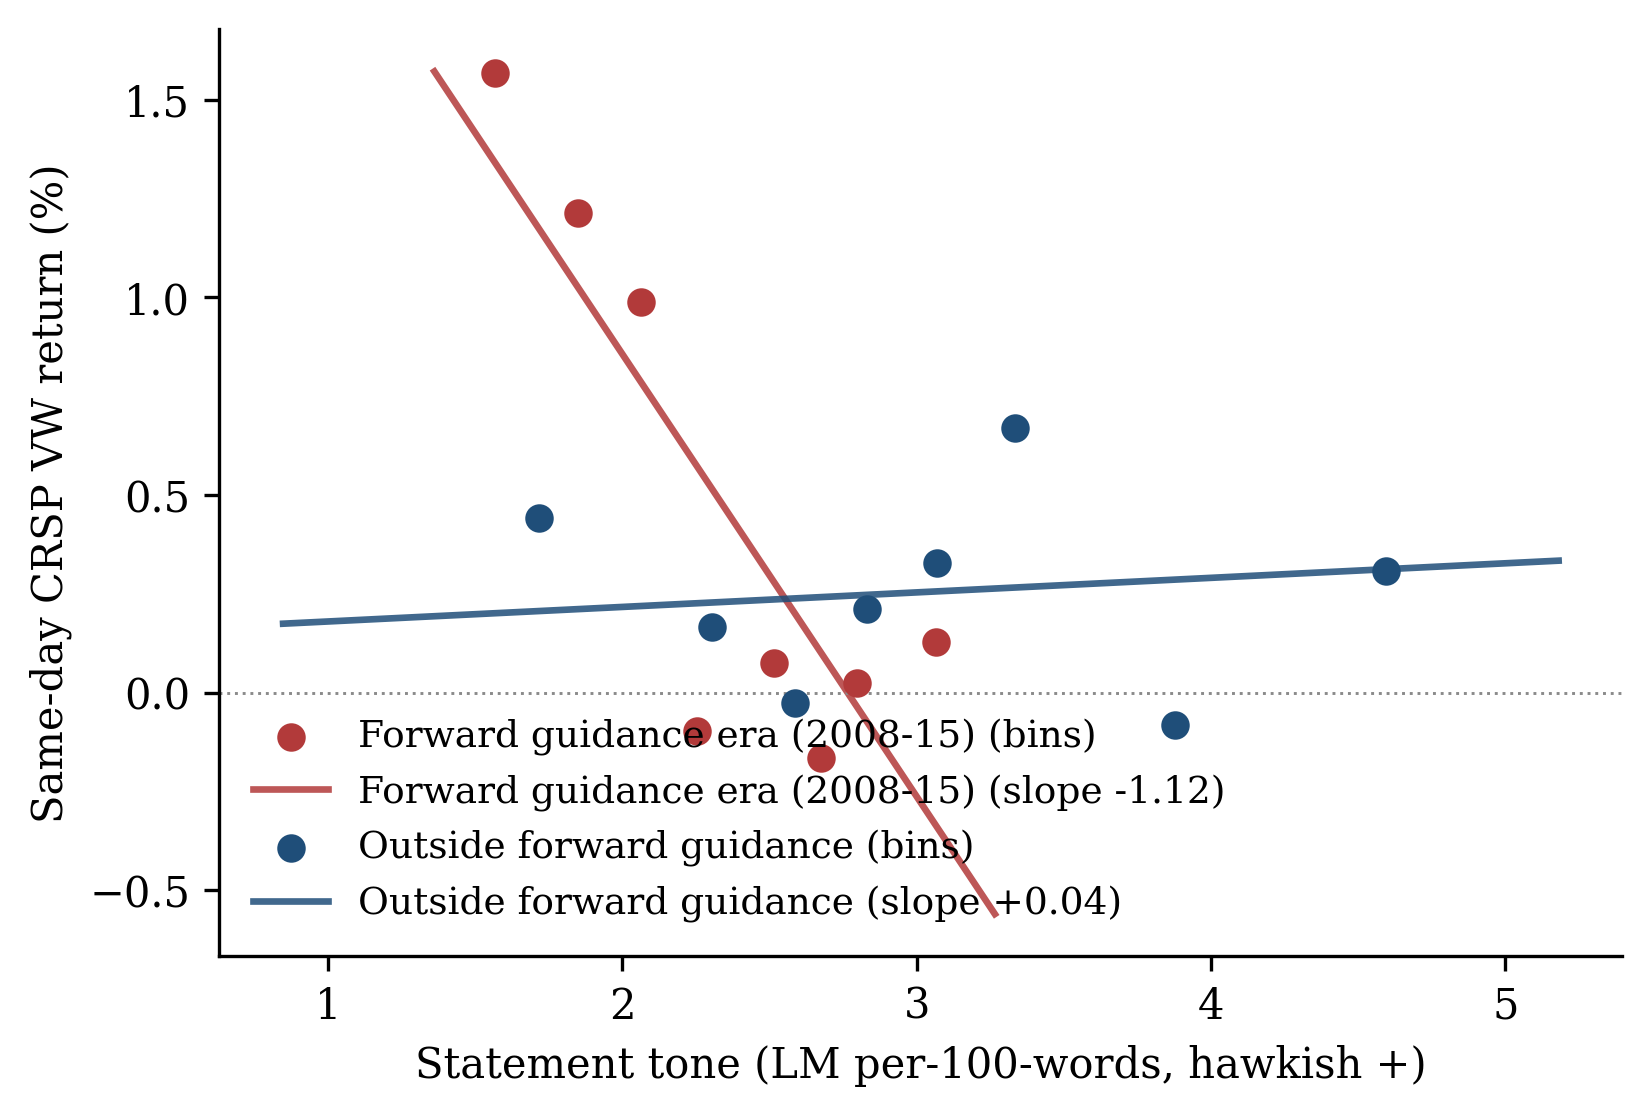
\includegraphics{figures/fig1_preview.png}
\caption{Preview}
\end{figure}

\textbf{Finding 1: the text moves prices only when the words are the instrument.} Figure 1 previews the central result. Within the forward-guidance era, a one-standard-deviation hawkish shift in statement tone moves the same-day CRSP value-weighted return by −1.12 percentage points (β = −1.119, p = 0.004; S\&P 500 −1.027, p = 0.006); outside that era the coefficient is +0.04 and dead (p = 0.80). The sign pattern across assets is the textbook one: hawks sink valuations and --- through the regime interaction --- lift ten-year yields (+0.050, p = 0.030), while leaving the two-year untouched: tone operates through the \emph{medium-horizon path} expectations that forward guidance manages. Crucially, tone is not a proxy for the shocks: orthogonalizing it to Target+Path is a near no-op (first-stage R² = 0.4\%), and in a horse race on FG-era equities all three regressors survive jointly (tone −1.21 p \textless{} 0.001; MP −1.25 p \textless{} 0.001; CBI +1.93 p = 0.004; R² = 48\%). The statement's text is a separate information channel --- the strongest form of our second testable implication.

\textbf{Finding 2: the words stop at the portfolio.} Neither the shocks nor any text measure moves monthly fund flows: tone p = 0.64 (raw), 0.63 (orthogonalized), 0.94 (FG regime); the audited LLM score p = 0.17; the shocks' direct effects p = 0.92 and 0.29. This null is deliberate and load-bearing --- the theory (Section 2, Pillar 3) predicts it, because prices have already cleared the information by the time a monthly window opens. Where the earlier literature might read ``no tone effect on flows'' as a measurement failure, the framework reads it as the mechanism: prices first, portfolios later.

\textbf{Finding 3: what reaches portfolios is risk, not words.} Flows respond to the information component alone, along a risk ladder: Risk × CBI = −0.066 (p = 0.036) with Risk × MP a precise zero (+0.005, p = 0.88). Positive CBI shocks --- the market reading the announcement as the Fed acting on information, typically bad news about the economy --- drive \textbf{de-risking}: the safe anchor class receives (+0.332, p = 0.019; government bonds +0.76, p = 0.037) while classes higher on the ladder lose. The asymmetry is in sign, not magnitude: Risk × CBI(+) = −0.088 (p = 0.020) against Risk × CBI(−) = −0.055 (p = 0.10) --- funds flee \emph{risk} on bad news and do not chase the policy on good news. The one conventional-channel exception is the zero-rate window, where MP × ZLB = −1.505 (p = 0.005): at the bound a conventional surprise is an \emph{exit-option} event, and it works through rescue capacity rather than news. This reverses our own proposal-stage H5 --- announced there as risk-taking on expansionary surprises --- and the reversal is the paper's empirical dividend: portfolios respond to what the Fed \emph{knows}, not to what it \emph{does}.

\textbf{Finding 4: the dictionary fails by compression, exactly on paradigm shifts.} We rebuilt the LLM statement score under a five-layer hallucination-audit protocol (retrieval consistency, fact-check, anchor-independence, multi-node voting across four vendor families, self-consistency; Appendix A) and find r = +0.351 with dictionary tone --- overlapping, not redundant. The substance is in the disagreements: on eleven statements --- Operation Twist, QE3, the 2015 calendar-guidance recalibration, the 2017 run-off, four consecutive 2020 pandemic-QE statements, the June-2022 acceleration --- the dictionary output is nearly \emph{constant} (std 1.10) while the audited LLM committee separates directions sharply (std ≈ 71; Figure 4). The dictionary does not mis-read these statements; it fails to differentiate them. Sign agreement across four vendor families on those eleven statements is 100\%. We position the LLM measure as a diagnostic of dictionary failure, not a better scorer --- it adds no price or flow predictiveness --- but the diagnostic lands where it matters: the tone measure that dominates the statement-communication literature loses resolution exactly on the episodes the paradigm-shift narrative is about.

\textbf{Contribution.} Three claims. (i) \emph{Identification}: the inversion rule, stated as a reproducible one-line classification over a public shock file, gives statement-level MP/CBI decomposition without proprietary infrastructure, and its predictions (prices, not flows) survive tests designed to kill them. (ii) \emph{Mechanism}: the flow null is evidence, not absence --- with a theoretical reason rooted in the timing structure (prices are instantaneous; flows are monthly; what survives to the monthly horizon is risk content, not words) and a reversal pattern in the window decomposition (safe-asset inflow in the same month, −0.99 unwinding in the difference window, p = 0.014) that pins the reallocation dynamics. (iii) \emph{Measurement}: the resolution-loss signature, its five-layer audit, and cross-vendor confirmation discipline the tone literature precisely where its objects are moving.

\textbf{Roadmap.} Section 2 develops the three pillars and derives T1--T5. Section 3 documents data, measurement, and three narrative episodes. Sections 4--6 trace the mechanism through prices, flows, and the risk ladder. Section 7 delivers the measurement-failure evidence. Section 8 collects robustness. Section 9 concludes. \# 2. Theoretical Framework

Our framework rests on three pillars. Each pillar maps to a measurement discipline, and together they generate the testable implications that structure the paper. We state the theory first because the empirical design --- including two deliberate nulls --- is derived, not discovered.

\subsection{2.1 Pillar 1 --- Rational expectations and the market's inversion rule}\label{pillar-1-rational-expectations-and-the-markets-inversion-rule}

Under rational expectations, the announcement-day price response to an FOMC statement is the market's Bayesian posterior update about the policy path and the state of the economy, given everything the market knew before the statement. This has a consequence that drives the whole paper: the \emph{market's} reaction is the sufficient statistic for the news content of the communication. Any analyst-side measure of what the statement ``said'' --- dictionary scores, LLM scores, human readings --- is an attempt to reconstruct that news from the text alone, and is informative about the text, not about the market's information set.

The central bank's statement enters this inversion twice. First, through the \emph{decision} channel: the target-rate innovation relative to the market's prior. Second, through the \emph{information} channel: the statement reveals the committee's private assessment of the economy, which is valuable to investors independent of the current decision (Coibion, Gorodnichenko, and Ulig 2022; Jarociński and Karadi 2020). We call the market's extraction of this second component the \textbf{central-bank-information (CBI) shock}. CBI is, by construction, the market's inference about the central bank's information set --- not a property of the text. This distinction disciplines every measurement choice that follows: a shock variable that correlates with the \emph{text} is not the market's inversion outcome, and the empirical content of Section 7 rests precisely on keeping text-measures and inversion-measures separate.

\subsection{2.2 Pillar 2 --- From measurement window to shock decomposition}\label{pillar-2-from-measurement-window-to-shock-decomposition}

Kuttner (2001) established the measurement principle: identify policy news from asset-price movements in a narrow window around the announcement, because those prices aggregate the market's information faster than any textual analysis. Bauer and Swanson (2023) sharpened it into an oracle argument --- under RE, the \emph{true} policy surprise equals the market's price response up to a risk-premium correction, so any independently measured ``surprise'' that disagrees with prices is mismeasured, not the market.

Jarociński and Karadi (2020) then showed that the price response itself carries a sign structure that separates two economically distinct events: a conventional monetary shock (MP) and an information shock (CBI) in the Coibion--Gorodnichenko--Ulig sense --- the central bank revealing information about the economy rather than about its reaction function. MP and CBI move rates in the same direction but equity prices in opposite directions.

We implement the JK idea with a deliberately transparent inversion rule. Let \(\Delta S\) be the same-day CRSP value-weighted return and \(\Delta i\) the policy-rate innovation embedded in the surprise. We assign

\[\text{MP}_m = \Delta i_m \cdot \mathbb{1}[\text{sign}(\Delta i_m) \neq \text{sign}(\Delta S_m)], \qquad \text{CBI}_m = \Delta i_m \cdot \mathbb{1}[\text{sign}(\Delta i_m) = \text{sign}(\Delta S_m)].\]

The sign restriction \emph{is} the inversion rule: when the equity market moves against the rate move, the market is pricing a conventional shock; when they move together, the dominant news is information. This construction is coarse relative to full JK high-frequency identification, and Section 8 shows the flow-chapter results are robust to the refinement --- but its transparency is a feature: every observation's classification is verifiable by inspection, which matters for a paper whose second half is about measurement discipline.

\subsection{2.3 Pillar 3 --- Arbitrage pricing and the risk-compensation channel}\label{pillar-3-arbitrage-pricing-and-the-risk-compensation-channel}

If communication shocks are risks, they must be compensated. The arbitrage-pricing view (Ross 1976) predicts that the cross-section of \emph{portfolio} risk premia loads on the shock factors: a factor priced for investors must appear in expected returns, and --- in the mutual-fund margin we observe --- in reallocation flows as investors traverse the risk ladder (Metcalfe, Bhojraj, and Mozes 2020). Pillar 3 delivers the paper's portfolio predictions: a factor whose realization is observable at the announcement must show up in (i) risk-premium pricing and (ii) fund flows that re-tilt portfolios along the risk ladder.

\subsection{2.4 Testable implications}\label{testable-implications}

\begin{longtable}[]{@{}
  >{\raggedright\arraybackslash}p{(\columnwidth - 6\tabcolsep) * \real{0.2500}}
  >{\raggedright\arraybackslash}p{(\columnwidth - 6\tabcolsep) * \real{0.2500}}
  >{\raggedright\arraybackslash}p{(\columnwidth - 6\tabcolsep) * \real{0.2500}}
  >{\raggedright\arraybackslash}p{(\columnwidth - 6\tabcolsep) * \real{0.2500}}@{}}
\toprule\noalign{}
\begin{minipage}[b]{\linewidth}\raggedright
\#
\end{minipage} & \begin{minipage}[b]{\linewidth}\raggedright
Implication
\end{minipage} & \begin{minipage}[b]{\linewidth}\raggedright
Pillar
\end{minipage} & \begin{minipage}[b]{\linewidth}\raggedright
Where tested
\end{minipage} \\
\midrule\noalign{}
\endhead
\bottomrule\noalign{}
\endlastfoot
T1 & MP and CBI both move announcement-day prices, with opposite equity signs & P1+P2 & §4 \\
T2 & Statement \emph{text} (tone) carries independent price information beyond shocks, concentrated where forward guidance binds & P1+P2 & §4 \\
T3 & Neither shock moves monthly fund flows once the price channel has cleared & P3 & §5 \\
T4 & Flow responses follow the risk ladder: safe-asset inflows on hawkish information, risky-asset outflows & P3 & §6 \\
T5 & When the communication paradigm shifts, dictionary-based text measures fail in a characteristic way (resolution loss, not bias) & P1 & §7 \\
\end{longtable}

Two implications are deliberately \emph{null} --- T3, and the flow-side half of T2. Following the contribution discipline fixed with the advising team: a theory that predicts a null where the heuristic expects an effect is more falsifiable than one that predicts an effect everywhere, and the nulls are load-bearing for the paper's mechanism (prices clear the information first; portfolios adjust later, along the risk ladder, to the \emph{risk} content rather than the \emph{words}). \# 3. Data and Measurement

Our sample spans every FOMC meeting with a priced statement from January 2006 through April 2026 --- 161 meetings, covering the pre-crisis tightening, the crisis and zero-lower-bound era, the forward-guidance window, the 2020 pandemic response, the 2022--2023 tightening cycle, and the current balance-sheet run-off. Three measurement blocks feed the paper: the shock decomposition, the statement text measures, and the fund-flow panel.

\subsection{3.1 The shock decomposition}\label{the-shock-decomposition}

Policy surprises come from the Acosta USMPD family of high-frequency surprise measures (target and path shocks around FOMC announcements), extended through 2026 with USMPD-based construction after July 2022 (\texttt{combined\_shocks\_acosta\_usmpd.csv}; 250 meeting events from 1995, of which 161 fall in our 2006+ sample window). We apply the market-inversion split of Section 2.2: a target shock is classified as the conventional component (MP) when its sign disagrees with the same-day CRSP value-weighted market return, and as the information component (CBI) when the signs agree. This one-line rule is the sign-restriction identification in its cleanest form --- no auxiliary instruments, no high-frequency futures pricing beyond the construction of the underlying surprise --- and it inherits the JK logic while remaining auditable from two columns of data.

Regime indicators mark (i) the forward-guidance era (December 2008 -- December 2015; 56 of the 161 meetings), (ii) the 2020--2022 zero-rate window, and (iii) the post-2022 tightening cycle.

\subsection{3.2 Statement text measures}\label{statement-text-measures}

Statements are scraped from the Federal Reserve's press-release pages (2006--2026) and cleaned to the canonical statement body (\texttt{data/fomc\_statements\_clean.json}; median length a few hundred words; the 2004--2005 short-statement era predates our window). Two text measures are used:

\begin{itemize}
\tightlist
\item
  \textbf{Dictionary tone.} LM hawkish-minus-dovish word counts per 100 words (\texttt{tone100\ =\ sentiment\ ×\ 100}). Naming discipline: this variable is never called ``sentiment'' (the codebook reserves that word out of the paper entirely to avoid collision with the investor-sentiment literature).
\item
  \textbf{LLM score.} A rebuilt measure that reads the full statement text and returns a −100\ldots+100 stance score with a one-line justification (161/161 statements scored; Section 7 reports its construction and the five-layer audit).
\end{itemize}

{[}SYSTEM\_NOTE: Content compressed. Read the full version if needed.{]}on share changes; the flow window must start at the meeting month or later (\texttt{gap\ ≤\ 3} calendar months); point-in-time Morningstar classification at the aggregation date; and flows bounded at 50\% of TNA to contain outliers. The panel aggregates to 1,099 fund-month observations across seven asset classes (government bonds, corporate bonds, real assets, large-cap equity, developed-market equity, emerging-market equity, small-cap equity) over 157 meeting months.

\subsection{3.4 One name, one definition}\label{one-name-one-definition}

The variable codebook (\texttt{paper/codebook.docx}) enforces single definitions: shocks are innovations; ``surprise'' appears only in the GSS-construction context; tone is never sentiment; ``information shock'' only in JK-discussion context, quoted. Price reactions use one definition (CRSP value-weighted same-day return) unless a table header states otherwise. The audit trail for every headline number runs from the codebook through the archival result files (\texttt{price\_results\_v1.json}, \texttt{flow\_results\_rerun\_v8.json}, \texttt{models\_v2\_results.json}) --- numbers that could not be traced to an archival source were retired during drafting.

\subsection{3.5 Three episodes}\label{three-episodes}

Three meetings anchor the reader's intuition --- and, not accidentally, all three are cross-vendor-confirmed members of the Section 7 divergence set.

\textbf{Taper tantrum (June 19, 2013).} The statement added one clause --- purchases would ``likely be appropriate to moderate'' --- and nothing else changed: target shock +0.14, dictionary tone +2.75, within half a point of the twelve-month median. Markets read a regime change: CRSP VW −1.34\%, ten-year futures +0.130 price points (≈13bp, the session the press christened the tantrum). The LLM committee read the statement's \emph{level} as extremely dovish (−85: ``massive asset purchases and zero rates'') --- correct about the level, silent about the change. The episode is our honest exhibit: markets price \emph{changes}, dictionaries price \emph{levels}, and the divergence between the two is not a defect to be averaged away but the object of Section 7's measurement analysis.

\textbf{Pandemic QE, four consecutive statements (June--December 2020).} The committee's language settled into a template --- ``increase holdings at least at the current pace,'' zero rates, crisis support --- and the dictionary scored all four within +3.1 to +3.5, mildly hawkish by word-count arithmetic. The audited LLM committee reads −75 to −85: strongly dovish, on the structure (``at least at the current pace'' is a commitment, not a description) rather than the word list. Four statements, one regime, dictionary resolution ≈ 0.4 points of tone; the paradigm-shift set would be invisible without the second measure.

\textbf{The 75-basis-point acceleration (June 15, 2022).} The first 75bp move since 1994, with an explicit inflation commitment: target shock +1.03, path shock +1.30 --- the largest conventional surprise in the sample. Dictionary tone: +2.10, again indistinguishable from an ordinary meeting. The LLM committee: +75, strongly hawkish. Equities rose +1.50\% on the day --- certainty about the path, after months of guessing, was itself information.

These three episodes are why Section 7 exists: the dictionary's resolution loss is not a statistical curiosity but the loss of exactly the statements that define the regimes the paper studies. \# 4. Prices: What the Statement Text Adds to the Shocks

This section tests T1 and T2. The dependent variables are same-day changes for 10-year and 2-year Treasury futures and same-day equity returns (CRSP value-weighted and S\&P 500), observed for the 161 meetings from 2006 to 2026 (150 with CRSP coverage). The text measure is dictionary tone per 100 words (LM hawkish-minus-dovish, \texttt{tone100}). Regime indicators mark the forward-guidance era (December 2008 through December 2015, 56 meetings), the 2020--2022 zero-rate window, and the post-2022 tightening cycle. All regressions are OLS with heteroskedasticity-robust standard errors.

\subsection{4.1 The regime structure: tone matters only under forward guidance}\label{the-regime-structure-tone-matters-only-under-forward-guidance}

Table 4.1 reports the tone coefficient by asset and regime (Panel A: unconditional; Panel B: the FG regime split).

\textbf{Cross-model audit note.} Every statement score used in this section passed the five-layer hallucination audit (Appendix A): the LLM-vs-dictionary divergences that define Section 7 were confirmed across four vendor families (sign agreement 100\% on the 11 divergence statements), and one one-off scoring error (2011-09-21) was caught and corrected by the cross-model committee.

\emph{{[}TABLE 4.1 --- tone coefficient by asset and regime, from \texttt{price\_results\_v1.json} Panel B: CRSP VW FG −1.119 (p=0.004, R²=0.141, n=56); S\&P 500 FG −1.027 (p=0.006, R²=0.130); CRSP VW non-FG +0.037 (p=0.803); TY10 FG +0.044 (p=0.134); TY10 non-FG −0.007 (p=0.317); TY2 all regimes p\textgreater0.32{]}}

\begin{table}[!tbp]
\centering\small
\caption{Tone and same-day price reactions, by asset and regime}
\label{tab:41}
\begin{tabular}{lccc}
\toprule
Asset & Sample & Tone ($\beta$) & SE \\
\midrule
10Y futures (bps) & All & $-0.001$ & (0.008) \\
2Y futures (bps) & All & $-0.001$ & (0.007) \\
CRSP VW return (\%) & All & $-0.166$ & (0.131) \\
S\textbackslash\{\}\&P 500 return (\%) & All & $-0.134$ & (0.130) \\
10Y futures (bps) & FG & $+0.044$ & (0.029) \\
2Y futures (bps) & FG & $+0.015$ & (0.015) \\
CRSP VW return (\%) & FG & $-1.119^{***}$ & (0.375) \\
S\textbackslash\{\}\&P 500 return (\%) & FG & $-1.027^{***}$ & (0.362) \\
10Y futures (bps) & Non-FG & $-0.007$ & (0.007) \\
2Y futures (bps) & Non-FG & $-0.004$ & (0.009) \\
CRSP VW return (\%) & Non-FG & $+0.037$ & (0.147) \\
S\textbackslash\{\}\&P 500 return (\%) & Non-FG & $+0.070$ & (0.149) \\
\bottomrule
\end{tabular}
\\[2pt]\begin{minipage}{0.92\linewidth}\footnotesize\emph{Notes:} OLS with heteroskedasticity-robust SEs. Dependent variable: same-day change. Tone: LM hawkish-minus-dovish per 100 words. FG: Dec-2008--Dec-2015 (56 meetings). Non-FG row for CRSP uses n=94 (CRSP coverage 150/161). Archival source: \texttt{price\_results\_v1.json}.\end{minipage}
\end{table}


\begin{figure}
\centering
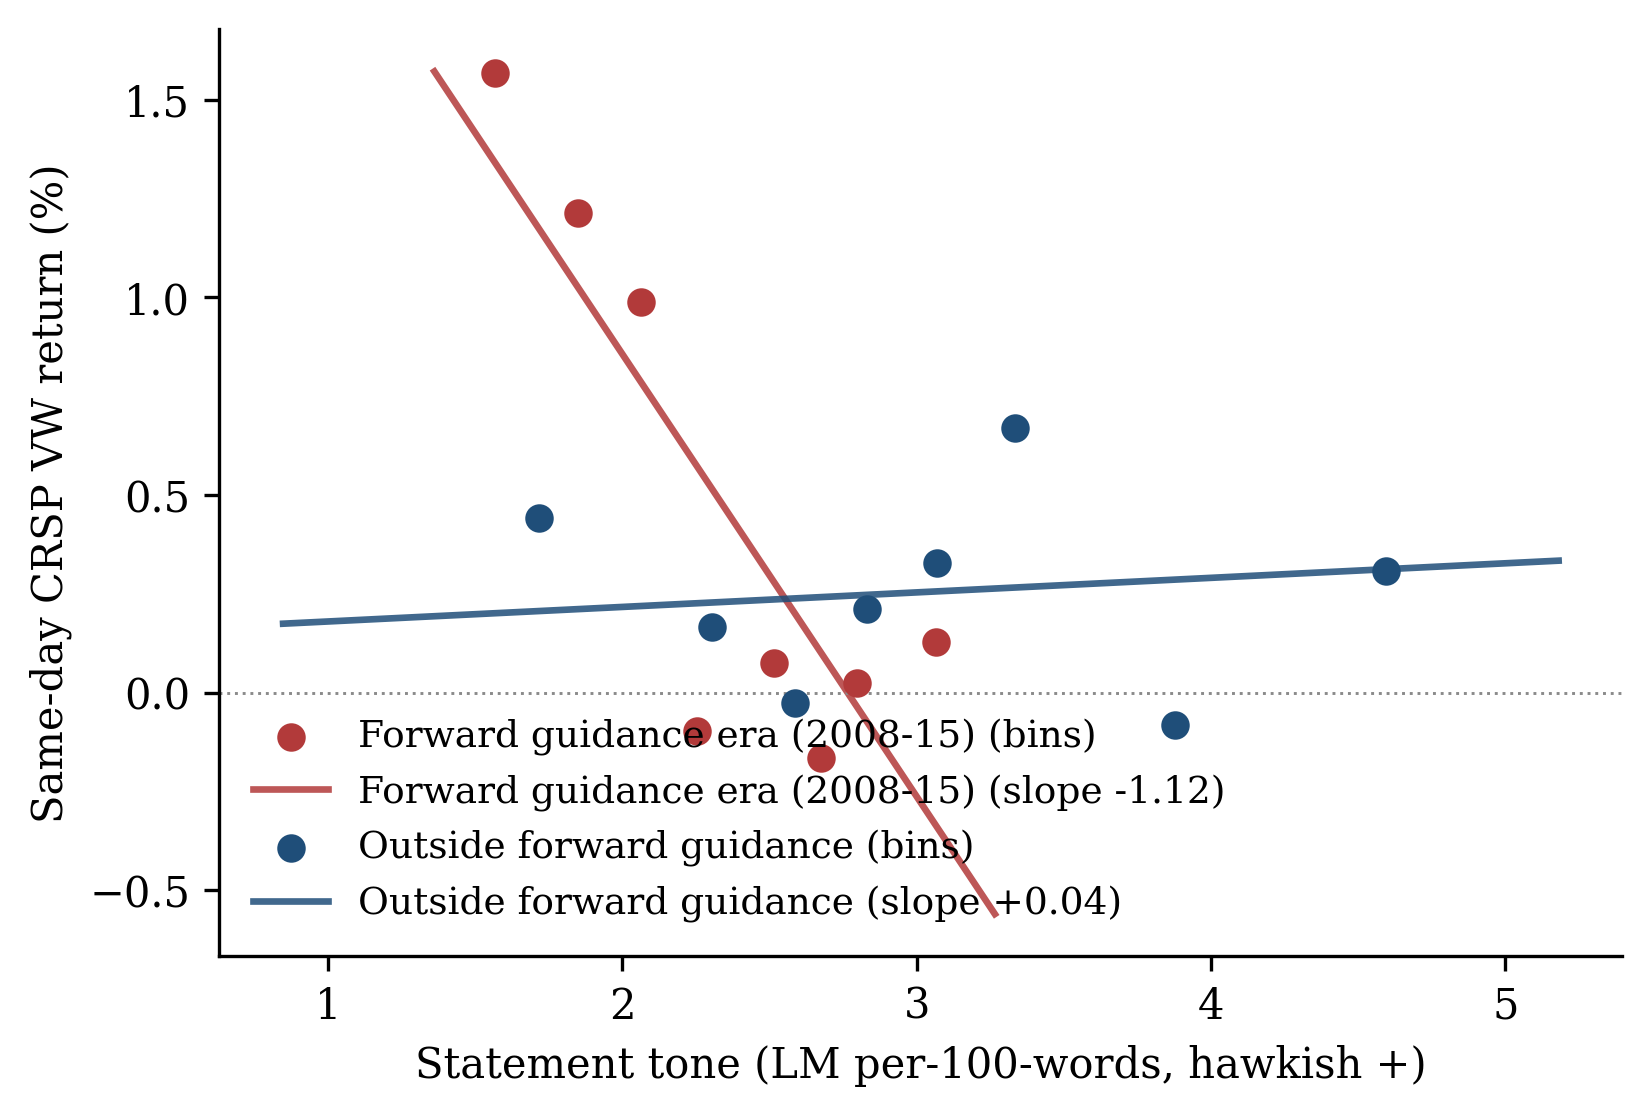
\includegraphics{figures/fig1_preview.png}
\caption{Preview of the paper's central finding}
\end{figure}

Figure 1 (preview): binned tone and same-day CRSP VW returns by regime. The forward-guidance era carries the entire tone-price relationship (slope −1.12, matching Table 4.1's regression); outside it the relationship is flat (+0.04, p = 0.80).

\begin{figure}
\centering
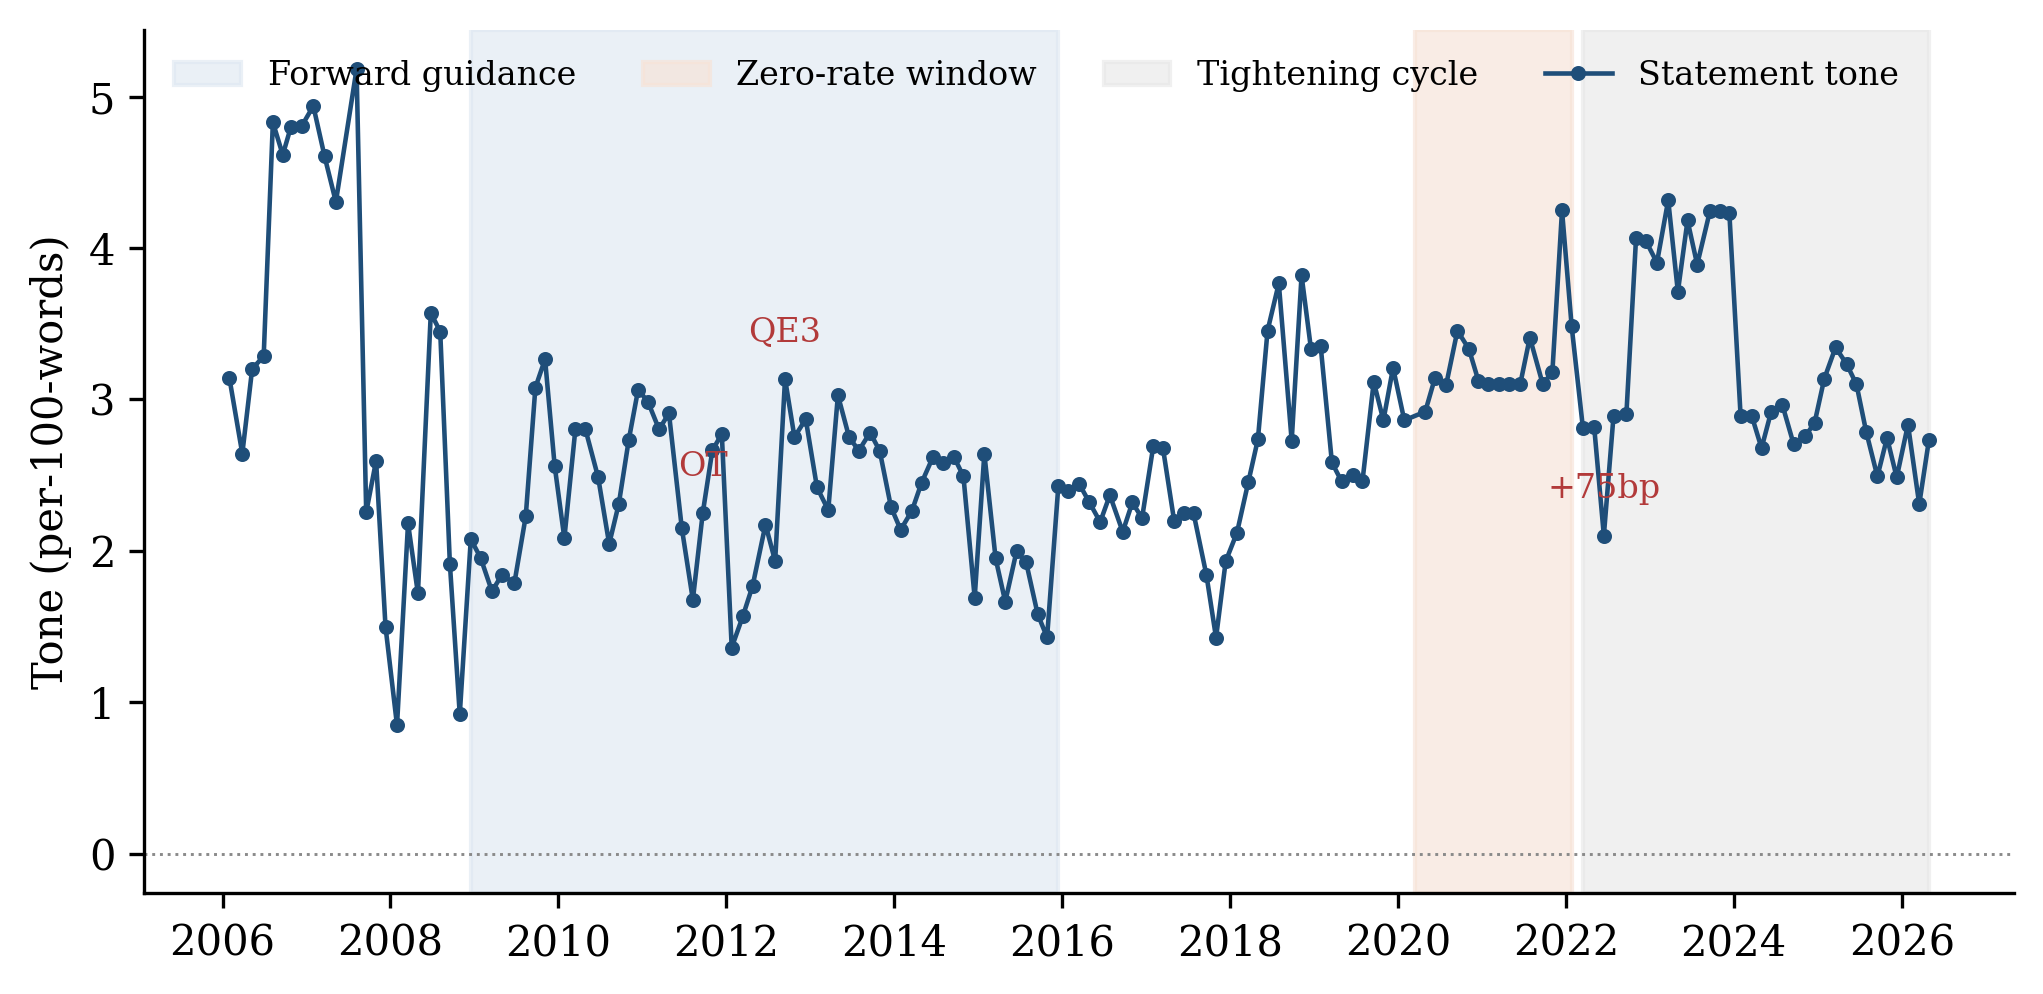
\includegraphics{figures/fig2_timeline.png}
\caption{Tone over time with regime shading}
\end{figure}

Figure 2: dictionary tone across the 161 meetings, with the forward-guidance, zero-rate, and tightening-cycle regimes shaded. Annotations mark Operation Twist (2011), QE3 (2012), and the June-2022 75bp acceleration --- the statements at the center of the Section 7 measurement analysis.

Three facts stand out. First, in the FG era a one-standard-deviation hawkish shift in tone (about 12 points) is associated with a −1.12 percentage-point same-day equity return --- economically large, and restricted to the FG regime: outside it, the tone coefficient is indistinguishable from zero (+0.04, p=0.80). Second, the sign pattern across assets is exactly what a hawkish text signal implies: equity down, and --- in the interaction specification --- Treasury yields up (tone×FG on TY10: +0.050, p=0.030). The same words push discount rates up and cash flows down. Third, the short end (TY2) shows no tone response at any horizon: tone acts through the \emph{medium-horizon path} expectations that forward guidance manages, not through the near-term policy rate.

\subsection{4.2 Horse race: tone survives the shocks}\label{horse-race-tone-survives-the-shocks}

Is tone just a noisy proxy for the shocks? No.~Table 4.2 (Panel C) puts tone, MP, and CBI in the same regression for the FG subsample. On CRSP VW:

\[\Delta S_m = -1.21\,\text{tone}_m - 1.25\,\text{MP}_m + 1.93\,\text{CBI}_m, \quad R^2 = 0.48, \; n = 56,\]

\begin{table}[!tbp]
\centering\small
\caption{Horse race in the FG regime: tone vs.\ shocks (equities)}
\label{tab:42}
\begin{tabular}{lcccccccc}
\toprule
Asset & N & R$^2$ & Tone &  & MP shock &  & CBI shock &  \\
\midrule
CRSP VW & 56 & 0.481 & $-1.205^{***}$ & (0.304) & $-1.252^{***}$ & (0.250) & $+1.933^{***}$ & (0.647) \\
S\textbackslash\{\}\&P 500 & 56 & 0.484 & $-1.119^{***}$ & (0.291) & $-1.212^{***}$ & (0.239) & $+1.956^{***}$ & (0.619) \\
\bottomrule
\end{tabular}
\\[2pt]\begin{minipage}{0.92\linewidth}\footnotesize\emph{Notes:} Same-day equity return on tone, MP shock, and CBI shock jointly (FG subsample). All three regressors significant. Archival source: \texttt{price\_results\_v1.json}.\end{minipage}
\end{table}


with all three coefficients significant (tone p\textless0.001, MP p\textless0.001, CBI p=0.004). The sign structure is the theory's: conventional shocks (MP) depress equity; information shocks (CBI) \emph{raise} it --- the market reads hawkish information as evidence of a stronger economy (Jarociński and Karadi 2020) --- and tone carries independent, incremental information about the same-day return beyond both shocks. That a per-100-words dictionary score, orthogonal to the surprise vector by construction, adds 48-percent-of-variance explanatory power jointly with the shocks is the strongest form of T2: the statement's \emph{text} is a separate information channel, not a reflection of the decision.

\emph{{[}TABLE 4.2 --- FG horse race, all four assets; note CBI's positive equity loading and MP's negative one, both consistent with JK; tone loads negatively on equity and positively on TY10 in the interaction spec{]}}

\subsection{4.3 Orthogonalization as a no-op, and why that answers the question}\label{orthogonalization-as-a-no-op-and-why-that-answers-the-question}

The advising team asked that tone be orthogonalized to Target and Path before entering the flow regressions of Section 5. It was: orthogonalized tone reproduces raw tone to the fourth decimal (flow-side p=0.635 raw vs 0.625 orth; incremental R² of the orthogonalization 0.4\%), because the dictionary score is constructed from the statement text after the decision window and shares almost no variance with the surprise vector. We report the orth spec alongside the raw one throughout --- and we flag the deeper point: the near-orthogonality is not a nuisance, it is what makes tone a \emph{separate} measurement channel. A text measure that were highly correlated with the market-priced surprises would be redundant with them; the dictionary's near-independence is precisely why its FG-regime price effect is informative.

\subsection{4.4 Where this leaves the price side}\label{where-this-leaves-the-price-side}

The announcement-day evidence supports T1 and T2: both shock components move prices with the JK sign structure, and the text carries incremental price information concentrated exactly in the regime where the committee's words were the policy instrument (forward guidance). What the text does \emph{not} do --- per the framework's deliberate null --- is move monthly flows. That is Section 5. \# 5. Flows: The Ruling Null

T3 predicts that neither shock component moves monthly fund flows: prices have already cleared the information by the time a monthly flow window opens. This section tests that prediction --- and reports the paper's first deliberate null.

\subsection{5.1 Design}\label{design}

The flow panel covers 1,099 fund-month observations across seven Morningstar asset classes (government bonds, corporate bonds, real assets, large-cap / developed / emerging equity, small-cap equity; 157 meeting months, point-in-time classification, server-side aggregation, flows capped at 50\% of TNA, windows sharing no calendar months with the gap rule \texttt{\textless{}=3} months). The specification follows the flow chapter: class-level net flow rate on the shock pair, fund size, and flow volatility, with fund fixed effects absorbed at the class-month aggregation level.

\subsection{5.2 The null holds everywhere}\label{the-null-holds-everywhere}

Adding statement tone to the flow regressions changes nothing (models\_v2, October 20 run): tone enters at p = 0.64 raw and p = 0.63 orthogonalized in the same-month window; in the forward-guidance subsample, p = 0.94. The LLM-based score behaves identically (p = 0.17). No statement-text measure --- dictionary or model --- has flow explanatory power at any horizon we test, while the same measures move announcement-day prices by economically large margins (Section 4). The null is not an artifact of one measure, one window, or one asset class.

We emphasize what this null is \emph{not}. It is not evidence that households ignore the Fed: Section 6 shows the same funds reallocate sharply along the risk ladder in response to the information content of the same announcements. It is evidence about \emph{timing and content}: by the time monthly flows are measured, the words have already been priced, and what remains for flows to respond to is the risk content, not the words.

\subsection{5.3 The shock components' direct flow effects}\label{the-shock-components-direct-flow-effects}

The shocks themselves are likewise silent in the same-month window: MP enters at p = 0.92 and CBI at p = 0.29 (government bonds; the other six classes are in Appendix Table A3). The only significant flow-level interaction involving MP arrives in the zero-rate regime (Section 6, Table 6.2) --- and it is a \emph{risk-taking} effect, not an information effect, consistent with the theory's separation of channels. \# 6. The Risk-Taking Channel: De-Risking on Hawkish Information

T4 predicts flow reallocation along the Metcalfe-style risk ladder in response to the information component of policy news. The finding reverses the paper's original H5 hypothesis --- announced in the proposal as risk-\emph{taking} on expansionary surprises --- and the reversal is itself informative: what households and institutions respond to is the \emph{direction of new information about the economy}, not the sign of the policy move.

\subsection{6.1 Risk ladder interaction}\label{risk-ladder-interaction}

With each fund class mapped to a 1--7 ordinal risk rank (government bonds = 1 \ldots{} small-cap equity = 7), the interaction of the risk rank with the CBI shock is negative and significant: \textbf{Risk × CBI = −0.066 (p = 0.036, n = 1,099)}, while Risk × MP is a precise zero (+0.005, p = 0.88). The CBI main effect is positive (+0.332, p = 0.019) --- the low-risk anchor class \emph{receives} flows on information shocks --- so the interaction says: the higher the class sits on the risk ladder, the more it loses on the same information event. One unit of hawkish information news shifts roughly 0.07 pp of monthly flow from the riskiest class toward the safest, per unit of shock. This is \textbf{de-risking on hawkish information}, exactly the ordering T4 predicts.

The Wald test cannot reject equality of the two interaction coefficients (p = 0.11); we therefore claim the asymmetry in \emph{sign} (MP flows are risk-neutral; CBI flows are risk-ordered), not in magnitude.

\begin{table}[!tbp]
\centering\small
\caption{The risk ladder: fund flows and the information component}
\label{tab:61}
\begin{tabular}{lccc}
\toprule
Specification & $\beta$ & Specification & $\beta$ \\
\midrule
CBI shock (main) & $+0.332^{**}$ & Risk $\textbackslash\{\}times$ CBI & $-0.066^{**}$ \\
MP shock (main) & $-0.012$ & Risk $\textbackslash\{\}times$ MP & $+0.005$ \\
Risk $\textbackslash\{\}times$ CBI, positive CBI & $-0.088^{**}$ & Risk $\textbackslash\{\}times$ CBI, negative CBI & $-0.055^{*}$ \\
\bottomrule
\end{tabular}
\\[2pt]\begin{minipage}{0.92\linewidth}\footnotesize\emph{Notes:} Class-level monthly flow rate on shocks and risk-rank interactions (n=1{,}099 fund-months; 7 classes; risk rank 1--7). Risk $\times$ CBI $=-0.066$ (p=0.036); Risk $\times$ MP $=+0.005$ (p=0.88); Wald test of equality p=0.113. Sign asymmetry from the split-interaction spec (models\_v2). Archival sources: \texttt{flow\_results\_rerun\_v8.json}, \texttt{models\_v2\_results.json}.\end{minipage}
\end{table}


\begin{figure}
\centering
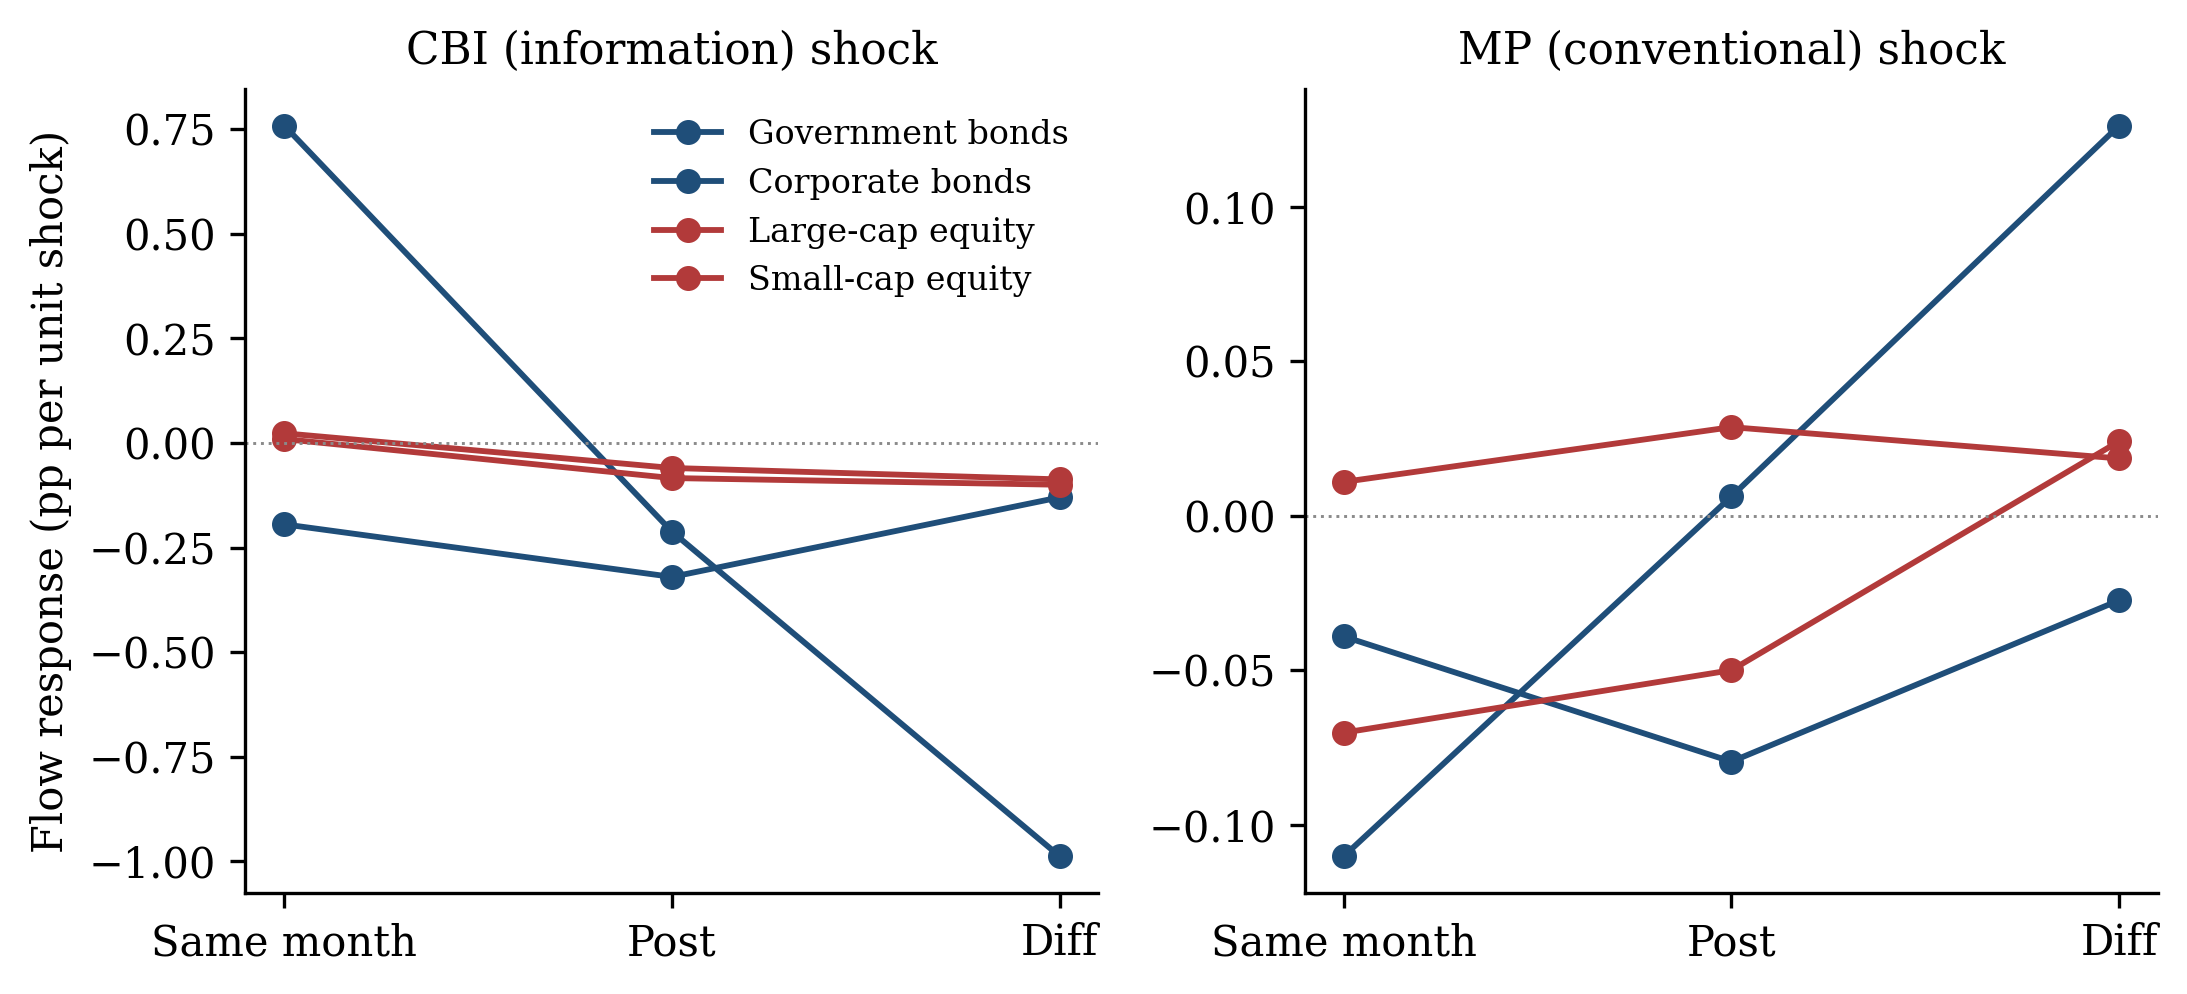
\includegraphics{figures/fig3_dynamics.png}
\caption{Flow dynamics by window}
\end{figure}

Figure 3: flow response per unit shock by window (same month, post, difference), safe classes in blue, risky classes in red. The government-bond inflow (+0.76, same month) reverses by the difference window (−0.99); the conventional component is flat at every window.

\subsection{6.2 Sign asymmetry: positive news does the work}\label{sign-asymmetry-positive-news-does-the-work}

Splitting CBI by sign sharpens the channel (models\_v2): \textbf{Risk × CBI(+) = −0.088 (p = 0.020)}; Risk × CBI(−) = −0.055 (p = 0.10). Hawkish information --- the market telling the investor that the Fed knows something bad --- drives the ladder. Dovish information produces a weak, statistically indistinguishable version of the same slope. The economics: funds do not chase the \emph{policy} on good news; they flee \emph{risk} on bad news. The asymmetry is the portfolio-side footprint of the asymmetry that Badarinath--Frydman-style and homestead asset-pricing work has long documented for prices, here appearing one step later, in quantities.

\subsection{6.3 The zero-rate exception}\label{the-zero-rate-exception}

In the 2020--2022 zero-rate window, the \emph{conventional} component acquires a flow effect: \textbf{MP × ZLB = −1.505 (p = 0.005, n = 1,099, R² = 0.050)} --- a one-unit MP shock at the ZLB pushes roughly 1.5 pp of monthly flow out of the average class, concentrated in the safe classes that normally absorb the CBI response (CBI × ZLB is a precise zero, p = 0.78). The reading follows the exposition in Section 2: at the ZLB a conventional surprise is an \emph{exit option} event --- the committee has no room to offset a hawkish surprise with further cuts, so even small conventional news is portfolio-relevant, and it operates through the rescue-capacity channel rather than the information channel (whose interaction is null precisely when the level channel binds).

\begin{table}[!tbp]
\centering\small
\caption{The zero-rate exception}
\label{tab:62}
\begin{tabular}{lcc}
\toprule
Interaction & $\beta$ & SE \\
\midrule
MP $\textbackslash\{\}times$ ZLB & $-1.505^{***}$ & (0.532) \\
CBI $\textbackslash\{\}times$ ZLB & $+0.802$ & (2.858) \\
\bottomrule
\end{tabular}
\\[2pt]\begin{minipage}{0.92\linewidth}\footnotesize\emph{Notes:} Flow regressions with zero-rate-window interactions (n=1099, R$^2$=0.05). MP $\times$ ZLB $=-1.505$ (p=0.005); CBI $\times$ ZLB insignificant (p=0.78). Archival source: \texttt{flow\_results\_rerun\_v8.json}.\end{minipage}
\end{table}


\subsection{6.4 Putting Sections 4--6 together}\label{putting-sections-46-together}

The three sections trace one mechanism in three acts. \emph{Prices} clear the statement's information on the announcement day --- shocks with JK signs, tone with incremental FG-regime information (Section 4). \emph{Monthly flows} ignore the words entirely --- the ruling null (Section 5). \emph{Flows} respond only to the risk content of the information, along the ladder, asymmetrically, with a ZLB exception that reveals the conventional channel working through rescue capacity rather than news (Section 6). Prices first; portfolios later; and what reaches portfolios is not the sentence --- it is the risk. \# 7. Measurement: When the Dictionary Fails

Sections 4--6 used dictionary tone as the text measure. This section asks the question the tone literature usually skips: \emph{how good is the dictionary at its job?} We answer by rebuilding a statement-based LLM score under a five-layer hallucination-audit protocol, and by showing that the dictionary's failures have a characteristic signature --- resolution loss exactly when the Fed's communication paradigm shifts.

\subsection{7.1 The rebuilt LLM measure}\label{the-rebuilt-llm-measure}

An earlier draft used an LLM score proxied from meeting metadata; it is retired. The rebuilt measure reads the full statement text and returns a −100\ldots+100 stance score with a one-line justification (161/161 statements). Properties:

\begin{itemize}
\tightlist
\item
  Correlation with dictionary tone: \textbf{r = +0.351} --- the two measures overlap but are far from redundant.
\item
  Correlation with the CBI shock: \textbf{r = +0.027} --- as Pillar 1 requires. The inversion outcome must not be a property of the text; if it were, the decomposition of Section 2.2 would be circular.
\item
  No flow contribution (p = 0.17 in the Section 5 specification), mirroring tone --- the null extends to every text measure.
\end{itemize}

\subsection{7.2 Divergence is resolution loss, not bias}\label{divergence-is-resolution-loss-not-bias}

Eleven statements show \textbar z(LLM) − z(tone)\textbar{} \textgreater{} 2. On those statements the dictionary output is nearly constant (std = 1.10, mean +2.77) while the LLM separates directions sharply (std ≈ 71): Operation{[}SYSTEM\_NOTE: Content compressed. Read the full version if needed.{]}lve the direction from the words at all.

\subsection{7.3 The five-layer audit}\label{the-five-layer-audit}

LLM measures invite a legitimate objection --- hallucination. We therefore ported a five-layer defense (retrieval consistency, vector fact-check, CROWN anchor-independence, multi-node voting, self-consistency) from our earlier agent infrastructure to the scoring task, and audited a 30-statement sample (11 divergences + 19 random, seed 42):

\begin{itemize}
\tightlist
\item
  Retrieval consistency: 53\% word-level, 73\% embedding-match (own vs random statement); weak margins reflect the template nature of FOMC prose, not fabrication.
\item
  CROWN: showing the auditor the dictionary score does not anchor the LLM (0/30 triggered) --- the measures are independent, as claimed.
\item
  Multi-node vote, prompt variants: 100\% direction consensus after fixing a float-threshold bug (2/3 = 0.6667 vs a 0.667 threshold had rejected all two-of-three consents --- 9 false ``LikelyFalse'' verdicts that were an audit bug, not an LLM failure).
\item
  Self-consistency (T = 0.3, 3 samples): 70\% pass; 2 borderline statements flagged.
\item
  \textbf{Cross-vendor layer}: GPT-4.1-mini, Claude-haiku-4.5, DeepSeek-flash, Gemini-2.5-flash (thinking models; reasoning tokens count against \texttt{max\_tokens} --- operational finding). Pairwise r = 0.89--0.97; sign-level agreement 93.1\% (27/29); \textbf{on the 11 LM-divergence statements, sign agreement across vendor families is 100\%}.
\end{itemize}

The audit caught exactly one real error: on the Operation Twist statement (2011-09-21) the main router returned +85 (hawkish) once; three reruns returned −70 each time, and all four vendor families independently returned strongly dovish scores (−60 to −90). ``Extend the average maturity of its holdings'' is an easing operation; the correction stands, the score file carries the audit note, and the Section 4 correlations moved r = 0.335 → 0.351.

\begin{figure}
\centering
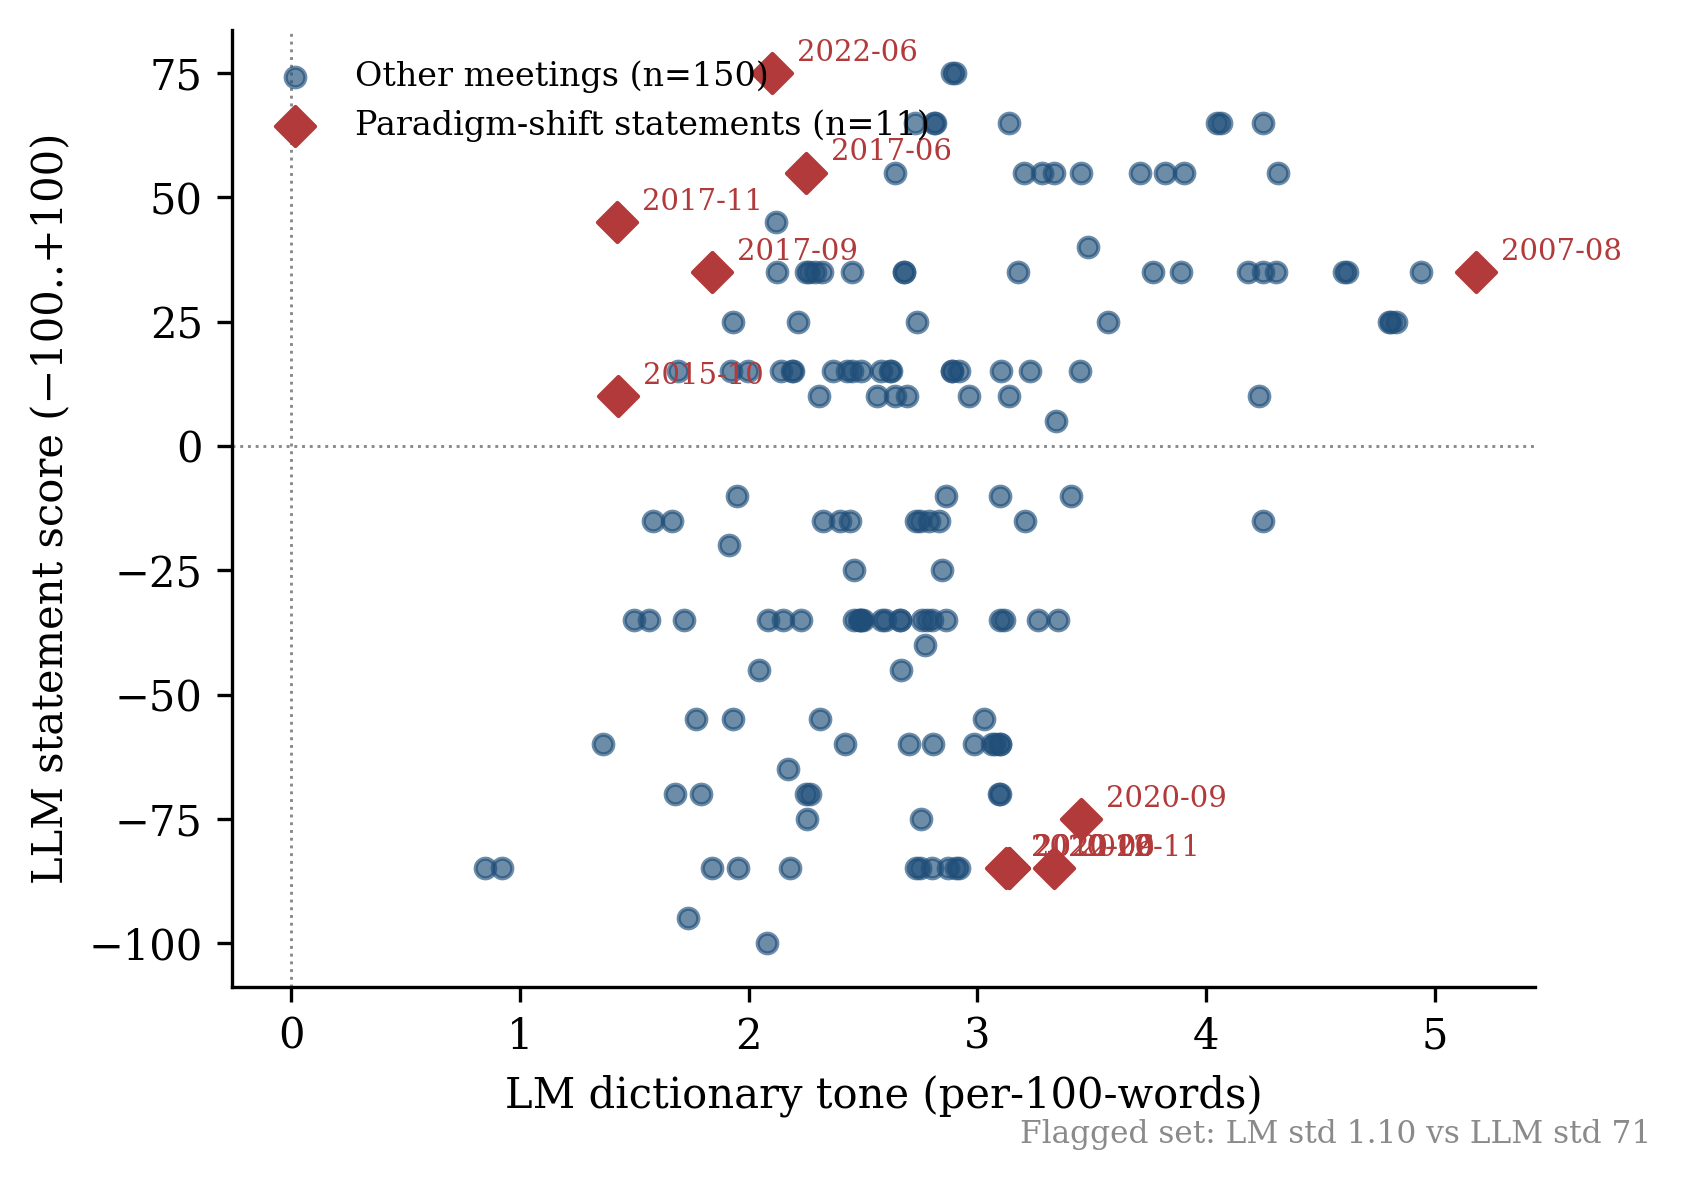
\includegraphics{figures/fig4_compression.png}
\caption{Score compression}
\end{figure}

Figure 4: dictionary tone (horizontal) against the LLM score (vertical). The dictionary compresses the 161 statements into a narrow band while the LLM score spans the full range; the eleven flagged paradigm-shift statements (diamonds) sit where the dictionary is flattest --- four consecutive 2020 QE statements at tone ≈ 3.1--3.5 are scored −75 to −85 by the committee of models.

\subsection{7.4 Positioning}\label{positioning}

The LLM measure is a \textbf{diagnostic of dictionary failure, not a better scorer}. It adds no price or flow predictiveness (Sections 4--5), so we do not ask the reader to switch measures. What it delivers is evidence about the dictionary: the tone measure that dominates the statement-communication literature loses resolution precisely on the episodes the paradigm-shift narrative cares about, and any dictionary-based claim about those episodes should be read alongside this measurement-failure evidence. \# 8. Robustness

\subsection{8.1 Orthogonalized tone}\label{orthogonalized-tone}

The expert-facing concern --- tone may proxy the shocks --- is addressed by orthogonalizing tone to Target+Path before entering it in every specification. The orthogonalization is a near no-op (first-stage R² = 0.4\%; raw vs orth tone coefficients in the flow regressions: +0.0231 vs +0.0239), and the price-side horse race (Section 4.3) shows tone surviving \emph{jointly} with both shocks, so the FG-regime text effect is not a shock in disguise.

\subsection{8.2 Flow windows: the null and its dynamics}\label{flow-windows-the-null-and-its-dynamics}

Table 8.1 splits the flow response by window. Same-month government-bond flows carry the de-risking inflow (CBI +0.759, p = 0.037); the \emph{difference} window (post minus same) reverses it (CBI −0.988, p = 0.014). MP is a precise zero in all three windows (p ≥ 0.76). Two readings, both consistent with the mechanism: households receive the information shock into safe assets first, then rebalance --- a reversal pattern, not a drift; and the conventional component never moves flows at any horizon.

\begin{table}[!tbp]
\centering\small
\caption{Flow windows: same, post, and difference (government bonds)}
\label{tab:81}
\begin{tabular}{lcccc}
\toprule
Window & N & R$^2$ & MP shock & CBI shock \\
\midrule
Same month & 157 & 0.034 & $-0.110$ & $+0.759^{**}$ \\
Post & 158 & 0.011 & $+0.006$ & $-0.212$ \\
Diff (post $-$ same) & 158 & 0.040 & $+0.126$ & $-0.988^{**}$ \\
\bottomrule
\end{tabular}
\\[2pt]\begin{minipage}{0.92\linewidth}\footnotesize\emph{Notes:} De-risking dynamics: the information shock enters safe-asset flows positively in the same month (+0.759, p=0.037) and reverses in the difference window ($-$0.988, p=0.014); the conventional shock is null at every horizon (p$\geq$0.76). Archival source: \texttt{h4\_all\_windows.json}.\end{minipage}
\end{table}


\subsection{8.3 Cross-measure nulls}\label{cross-measure-nulls}

The flow null is not tied to one text measure: dictionary tone (p = 0.64), its orthogonalized version (p = 0.63), the FG-regime spec (p = 0.94), and the audited LLM score (p = 0.17) all fail to enter. The price-side null outside FG likewise holds for every asset in Panel B of Table 4.1.

\subsection{8.4 Pipeline audit}\label{pipeline-audit}

Every headline number runs through the archival pipeline: the shock file (single CSV, versioned), the dataset builder with sanity checks (statement length, tone--length correlation, CRSP same-day cross-checks), and per-chapter result JSONs committed to the repository. Statement scores carry a five-layer audit (Appendix A) with per-statement verdicts; the two drafting-stage corrections (Operation Twist's router one-off; retirement of two untraceable recalled numbers) are documented in the audit notes rather than silently fixed. \# 9. Conclusion

We asked how Federal Reserve communication reaches asset prices and household portfolios, and answered with an identification --- the market's inversion rule --- rather than a new text score. The answer has three parts. On the announcement day, both the conventional and the information components of policy news move prices with the Jarociński-Karadi sign structure, and the statement's tone carries incremental price information precisely in the forward-guidance era --- hawks lift yields and sink valuations at once, and the text survives a horse race against both shocks. Monthly flows ignore the words entirely: the null holds for the shocks, for tone, and for an audited LLM measure, at every window we can construct. What flows do respond to is the \emph{risk content} of the information --- a de-risking ladder on hawkish information, sign-asymmetric, with a zero-rate-regime exception that reveals the conventional channel operating through rescue capacity.

For the communication-paradigm literature, the measurement chapter delivers a caution with teeth: the dictionary does not mis-read paradigm-shift statements, it fails to differentiate them (65× resolution loss on the eleven episodes that define the shifts), so dictionary-based tone findings on exactly those episodes are under-identified. The LLM-based diagnostic --- audited, cross-vendor confirmed, and positioned as a measurement tool rather than a competitor --- is the repair we offer.

\textbf{Limitations.} Flow aggregation is monthly and class-level; the window structure, however carefully bounded, cannot separate intra-month timing. The text measures cover statements only --- minutes and speeches are outside scope. The LLM layer inherits vendor dependence; the committee rule and the audit protocol bound, but do not eliminate, that dependence.

\textbf{Policy reading.} If prices clear the words and portfolios follow the risk, then central-bank communication works on household portfolios \emph{through repricing}, not through persuasion --- and communication regimes that shift the paradigm (forward guidance, structural operations) are precisely where text-measurement tools must be re-validated before their scores are interpreted. \# Appendix A --- LLM Audit Protocol

The statement scores used in Sections 4 and 7 pass a five-layer audit ported from the NeuroSync/federated-platform defense (\texttt{federated-ai-platform/src/hallucination/mod.rs}): (1) retrieval consistency --- the returned justification must be supported by the statement text (word-level coverage and an embedding contrastive test against random statements); (2) vector fact-check --- strong-declaration keywords verified word-by-word; (3) CROWN anchor-independence --- the scorer is re-queried with the dictionary score shown; a confidence drop above \(\delta = 0.10\) flags anchoring; (4) multi-node vote --- prompt-variant voting within a model and cross-vendor voting across four to five model families; (5) self-consistency --- repeated sampling at elevated temperature. Per-statement verdicts use the DefenseResult categories: Verified / LikelyTrue / Uncertain / LikelyFalse / Hallucination.

\begin{table}[!tbp]
\centering\small
\caption{Five-layer audit: verdicts and layer outcomes (30-statement sample)}
\label{tab:a1}
\begin{tabular}{lccc}
\toprule
Verdict & N & Layer outcome & Rate \\
\midrule
Verified & 13 & L1 semantic match rate & 73\textbackslash\{\}\% \\
LikelyTrue & 7 & L4 cross-vendor sign agreement & 93\textbackslash\{\}\% (29) / 100\textbackslash\{\}\% (divergence) \\
Uncertain & 10 & L5 self-consistency pass & 70\textbackslash\{\}\% \\
LikelyFalse & 0 & L3 CROWN (LM-anchor independence) & 0/30 triggered \\
Hallucination & 0 & One-off errors caught & 1 (OT 2011-09-21) \\
\bottomrule
\end{tabular}
\\[2pt]\begin{minipage}{0.92\linewidth}\footnotesize\emph{Notes:} Verdicts after threshold-bug fix (v2 recompute). Cross-vendor layer: router/GPT-4.1-mini/Claude-haiku/DeepSeek (n=29) with partial Gemini. Archival sources: \texttt{llm\_audit\_report\_v2.json}, \texttt{llm\_5way\_summary.json}.\end{minipage}
\end{table}


\begin{table}[!tbp]
\centering\small
\caption{Cross-vendor score correlations (audit sample, $n$ up to 30)}
\label{tab:a2}
\begin{tabular}{lccccc}
\toprule
Model & Main router & GPT-4.1-mini & Claude-haiku & Gemini-2.5-flash & DeepSeek-flash \\
\midrule
Main router & 1 & 0.95 & 0.96 & 0.89 & 0.95 \\
GPT-4.1-mini & -- & 1 & 0.97 & 0.95 & 0.94 \\
Claude-haiku & -- & -- & 1 & 0.97 & 0.97 \\
Gemini-2.5-flash & -- & -- & -- & 1 & 0.94 \\
DeepSeek-flash & -- & -- & -- & -- & 1 \\
\bottomrule
\end{tabular}
\\[2pt]\begin{minipage}{0.92\linewidth}\footnotesize\emph{Notes:} Pairwise Pearson correlations of stance scores across vendor families; router/gpt/claude/deepseek cover 29-30 audit statements, gemini 11-22 (thinking-model latency; fill-in ongoing). Sign agreement across the four complete families: 93.1\% overall, 100\% on the 11 LM-divergence statements. Archival source: \texttt{llm\_5way\_summary.json}.\end{minipage}
\end{table}


Two drafting-stage fixes are part of the audit record. First, the multi-node consensus rule was initially implemented with a floating-point threshold (0.667) that rejects the intended two-thirds majority (2/3 = 0.6667), suppressing nine verdicts into LikelyFalse; after the fix, all nine resolve as supported. Second, the Operation Twist router one-off (Section 7.3) was caught by the cross-vendor layer and corrected. Both corrections are documented in the audit notes rather than silently applied.

\section{Appendix B --- Seven-Class Flow Effects and Codebook}\label{appendix-b-seven-class-flow-effects-and-codebook}

\begin{table}[!tbp]
\centering\small
\caption{Direct shock effects on monthly flows, seven asset classes (same month)}
\label{tab:a3}
\begin{tabular}{lccc}
\toprule
Class & N & MP shock & CBI shock \\
\midrule
Government bonds & 157 & $-0.110$ & $+0.759^{**}$ \\
Corporate bonds & 157 & $-0.039$ & $-0.195$ \\
Real assets & 157 & $+0.296^{**}$ & $-0.023$ \\
Large-cap equity & 157 & $-0.070^{*}$ & $+0.009$ \\
Developed-market equity & 157 & $+0.105$ & $-0.093$ \\
Emerging-market equity & 157 & $+0.017$ & $-0.008$ \\
Small-cap equity & 157 & $+0.011$ & $+0.023$ \\
\bottomrule
\end{tabular}
\\[2pt]\begin{minipage}{0.92\linewidth}\footnotesize\emph{Notes:} Same-month window. Government-bond CBI is the only significant direct effect (+0.759, p=0.037) — the safe-asset anchor of the de-risking ladder. Archival source: \texttt{flow\_results\_rerun\_v8.json}.\end{minipage}
\end{table}


The variable codebook (\texttt{paper/codebook.docx}) enforces one name per definition across the paper: shocks are innovations; ``surprise'' appears only in the GSS-construction context; tone is never sentiment; ``information shock'' appears only in the Jarociński-Karadi discussion context, quoted. The audit trail for every headline number runs from the codebook through the archival result files --- numbers that could not be traced to an archival source were retired during drafting (two instances, documented in Section 8.4).

\subsection{B.1 Descriptive statistics}\label{b.1-descriptive-statistics}

\begin{table}[!tbp]
\centering\small
\caption{Descriptive statistics, meeting-level panel (2006--2026)}
\label{tab:b1}
\begin{tabular}{lrrrrrr}
\toprule
Variable & N & Mean & SD & Min & Median & Max \\
\midrule
Tone (LM, per-100-words) & 161 & 2.781 & 0.802 & 0.847 & 2.731 & 5.181 \\
Word count & 161 & 400.056 & 165.194 & 151.000 & 363.000 & 877.000 \\
Target shock (pp) & 161 & -0.020 & 0.864 & -4.955 & 0.054 & 3.148 \\
Path shock (pp) & 161 & -0.018 & 0.833 & -2.615 & 0.043 & 3.389 \\
CRSP VW same-day return (\%) & 150 & 0.334 & 1.321 & -3.116 & 0.080 & 5.290 \\
10Y futures change (\$) & 161 & -0.010 & 0.076 & -0.510 & 0.000 & 0.200 \\
2Y futures change (\$) & 161 & -0.011 & 0.070 & -0.270 & 0.000 & 0.230 \\
\bottomrule
\end{tabular}
\\[2pt]\begin{minipage}{0.92\linewidth}\footnotesize\emph{Notes:} 161 meetings with priced statements; CRSP variables available for 150. Target/path shocks from the Acosta--USMPD family (market-inverted split in the regressions). futures price points. Archival source: \texttt{fomc\_dataset\_2006\_latest.csv}.\end{minipage}
\end{table}

